%%=============================================================================
%% CAPITULO 2 -- REFERENCIAL TEORICO
%%
%% Esta e a parte do trabalho que mais demanda dominio das regras de citacao
%% (diretas e indiretas). Reveja a NBR 10520 antes de escrever.
%%=============================================================================

\section{Referencial teórico}

Texto introdutório de um parágrafo, conforme exigido pela ABNT. Essa parte do
trabalho demanda o domínio das regras de citação (diretas e indiretas). É nessa
parte do trabalho que problemas legais em relação à apropriação de ideias de
outros autores ocorrem com maior frequência. Portanto, reveja as regras
estabelecidas pela ABNT para citações diretas e indiretas e para a indicação de
fontes de gráficos, figuras ou outro recurso ilustrativo utilizado.

É importante lembrar que o desenvolvimento do trabalho será guiado pelo
orientador, a quem cabe julgar se a Seção 2 poderá iniciar-se por ``revisão de
literatura'', ``referencial teórico'' ou já abordar o primeiro tema a ser
discutido no trabalho. O número de subtópicos desse item dependerá dos conceitos
envolvidos na sua questão problema.

%% --- Exemplo de figura com legenda ACIMA e fonte ABAIXO --------------------
\begin{figure}[htb]
  \caption{Título da Figura}
  \label{fig:exemplo}
  \centering
  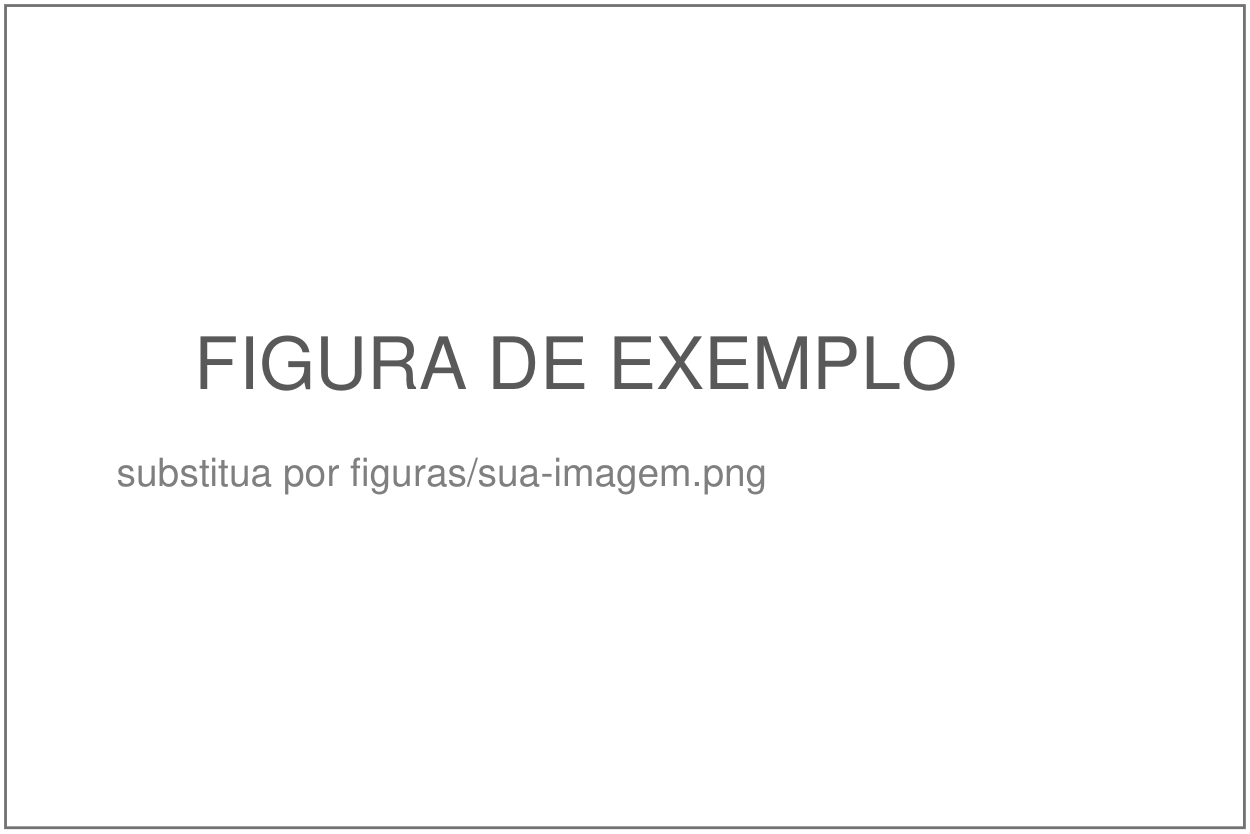
\includegraphics[width=0.6\textwidth]{figuras/exemplo-figura.png}
  \fonte{Niemeyer (2008).}
\end{figure}

Caso a ilustração seja de sua autoria, escreva \textbf{Fonte:} Do autor
(\the\year). Use o mesmo padrão para quadros e gráficos, alterando apenas o
título. Se precisar de notas de rodapé\footnote{Texto de exemplo para nota de
rodapé. A nota de rodapé apresenta informações ou comentários adicionais sobre o
conteúdo, em fonte 10 e espaçamento simples.}, elas devem estar dispostas no pé
da página.

\subsection{Título representativo do primeiro conceito: subtítulo se houver}

Discussão específica sobre a articulação das informações com foco na delimitação
proposta pelos cursistas (bibliografia e orientação a cargo dos orientadores
acadêmicos).

\subsubsection{Título representativo: subtítulo se houver}

No decorrer do desenvolvimento de cada capítulo (seção) e subcapítulo (subseção)
utilizam-se citações diretas e indiretas para esclarecimentos, sustentações ou
ilustrações de determinado assunto. A citação direta é a transcrição textual, sem
alteração, de parte da obra do autor consultado.

\textbf{Exemplo: citação direta de até 3 linhas} --- vai entre aspas duplas, no
corpo do parágrafo:

De acordo com \citeonline[p.~35]{sa1971}, acontece ``por meio da mesma arte de
conversação que abrange tão extensa e significativa parte da nossa existência
cotidiana''.

\textbf{Exemplo: citação direta com mais de 3 linhas} --- recuo de 4~cm, fonte
10, espaçamento simples e sem aspas:

Assim, de acordo com Nicholls:

\begin{citacao}
A teleconferência permite ao indivíduo participar de um encontro nacional ou
regional sem a necessidade de deixar seu local de origem. Tipos comuns de
teleconferência incluem o uso da televisão, telefone e computador. Através de
áudio-conferência, utilizando a companhia local de telefone, um sinal de áudio
pode ser emitido em um salão de qualquer dimensão. \parencite[p.~181]{nicholls1993}
\end{citacao}

\textbf{Exemplo: citação indireta} --- é o texto baseado na obra do autor
consultado; você transcreve aquilo que entendeu do texto lido:

Para \citeonline{authier1982}, a ironia seria assim uma forma implícita de
heterogeneidade. Para mais informações sobre citação, consulte a norma
NBR 10520 \parencite{abnt10520}.

%% --- Exemplo de quadro -----------------------------------------------------
\begin{quadro}[htb]
  \caption{Título do quadro}
  \label{qua:exemplo}
  \centering
  \begin{tabular}{ll}
    \toprule
    \textbf{Elemento} & \textbf{Norma aplicável} \\
    \midrule
    Trabalhos acadêmicos & NBR 14724 \\
    Referências          & NBR 6023  \\
    Citações             & NBR 10520 \\
    Sumário              & NBR 6027  \\
    Resumo               & NBR 6028  \\
    \bottomrule
  \end{tabular}
  \fonte{Elaborado pelo autor (\the\year).}
\end{quadro}

%% --- Exemplo de tabela -----------------------------------------------------
\begin{table}[htb]
  \caption{Nome da Tabela 1}
  \label{tab:exemplo}
  \centering
  \begin{tabular}{lrr}
    \toprule
    \textbf{Categoria} & \textbf{Frequência} & \textbf{\%} \\
    \midrule
    Categoria A & 120 & 40,0 \\
    Categoria B &  90 & 30,0 \\
    Categoria C &  90 & 30,0 \\
    \midrule
    \textbf{Total} & \textbf{300} & \textbf{100,0} \\
    \bottomrule
  \end{tabular}
  \fonte{Dados da pesquisa (\the\year).}
\end{table}

%% --- Exemplo de grafico ----------------------------------------------------
\begin{grafico}[htb]
  \caption{Nome do Gráfico 1}
  \label{gra:exemplo}
  \centering
  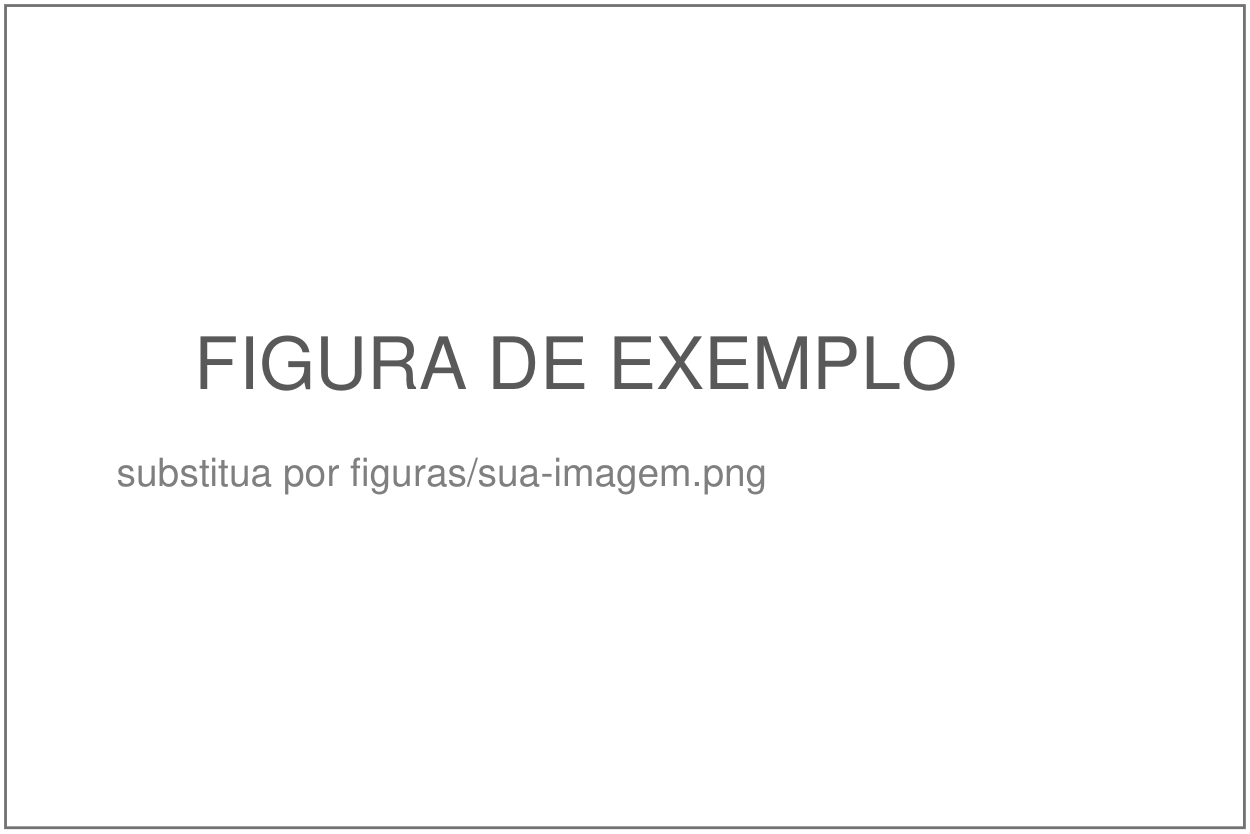
\includegraphics[width=0.55\textwidth]{figuras/exemplo-figura.png}
  \fonte{Elaborado pelo autor (\the\year).}
\end{grafico}
